\section{\benchmarkName{}}
\label{sec:SkillsBench}

We present \benchmarkName{}, a benchmark for evaluating the efficacy of \emph{Skills augmentation} in LLM-based agents. Built on the Harbor framework~\citep{merrill2026terminalbenchbenchmarkingagentshard, harborframeworkteam2026harborframework}, each task adopts a containerized structure with an environment that includes agent Skills and related data, a deterministic verification test, and an oracle solution. Following best practices for agentic benchmarks~\citep{zhu2025bestpractices, anthropic2026demystifying}, we ensure strict isolation and deterministic verification. Unlike Terminal-Bench, which evaluates raw model and agent harness capability, \benchmarkName{} introduces a key methodological difference: we evaluate every task under both \emph{vanilla} (no Skills) and \emph{Skills-augmented} conditions, enabling direct measurement of Skills efficacy.

\subsection{Skills Specification}
\label{sec:skill_spec}

A \textbf{Skill} is an artifact that satisfies four criteria:
\begin{itemize}[nosep,leftmargin=*]
    \item \textbf{Procedural content}: Contains how-to guidance (procedures, workflows, SOPs), not factual retrieval
    \item \textbf{Task-class applicability}: Applies to a class of problems, not a single instance
    \item \textbf{Structured components}: Includes a \texttt{SKILL.md} file plus optional resources (scripts, templates, examples)
    \item \textbf{Portability}: Skills are soley based on file systems, so it's easy to edit, version, share, and be used across different skills-compatible agent harnesses. 
\end{itemize}

\noindent This definition explicitly \emph{excludes}: system prompts (lack structure and resources), few-shot examples~\citep{brown2020languagemodelsfewshotlearners} (declarative, not procedural), RAG retrievals~\citep{lewis2021retrievalaugmentedgenerationknowledgeintensivenlp} (factual, not procedural), and tool documentation~\citep{schick2023toolformerlanguagemodelsteach, qin2024toolllm} (describes capabilities, not procedures).
We acknowledge this boundary is not absolute
(for example, a StackOverflow answer may blend factual and procedural content),
but our criteria provide operational clarity for benchmark construction.
We highlight the distinguishing features of Skills compared to other augmentation paradigms in \autoref{tab:comparison}.


% \paragraph{Skills Structure.}
In \benchmarkName{}, each Skill is a modular package located in \texttt{environment/skills/} containing:
\begin{itemize*}%[nosep,leftmargin=*]
    \item \texttt{SKILL.md}: Natural language instructions specifying \emph{how} to approach a class of tasks,
    i.e., workflows, standard operating procedures, or domain conventions.
    \item \textbf{Resources}: Executable scripts, code templates, reference documentation, or worked examples that the agent may invoke or consult.
\end{itemize*}

% \paragraph{Comparison with Related Concepts.}
% Table~\ref{} distinguishes Skills from related augmentation paradigms.

\begin{table}[t]
\centering
\small
\caption{Comparison of runtime augmentation paradigms. Skills uniquely combine modular packaging with procedural guidance and optional executable resources, while remaining portable across models and harnesses.}
\label{tab:comparison}
\begin{tabular}{lcccc}
\toprule
& \textbf{Prompts} & \textbf{RAG} & \textbf{Tools} & \textbf{Skills} \\
\midrule
Modular/reusable & \texttimes & \checkmark & \checkmark & \checkmark \\
Procedural guidance & Limited & \texttimes & \texttimes & \checkmark \\
Executable resources & \texttimes & \texttimes & \checkmark & \checkmark \\
Cross-model portable & \checkmark & \checkmark & \checkmark & \checkmark \\
\bottomrule
\end{tabular}
\end{table}

\subsection{Task Specification}

Each task in \benchmarkName{} is a self-contained module comprising four components:
% \vspace{-1.95em}
\begin{itemize}[nosep,leftmargin=*]
\item \textbf{Instruction.} A human-readable task description specifying the objective, input format, and expected output. We write instructions to be solvable by a knowledgeable human without access to the paired Skills, though the Skills may substantially reduce time-to-solution.

\item \textbf{Environment.} A Docker container with task-specific data files and a \texttt{skills/} subdirectory containing modular Skills packages. The container ensures reproducibility through isolated dependencies and clean file system state.

\item \textbf{Solution.} A reference implementation demonstrating the task's resolvability. This oracle validates that each task has at least one correct solution path.

\item \textbf{Verifier.} Deterministic test scripts with programmatic assertions, including numeric tolerances where appropriate. This ensures reproducible pass/fail determination without LLM-as-a-judge variance, following execution-based evaluation best practices~\citep{wang2023execution, brown_verifiers_2025}.
\end{itemize}
\subsection{Dataset Construction}
The expressive and flexible nature of Skills and our task specifications enables broad coverage across diverse domains and problem types such as ....
To maximize this diversity, we adopted a \textbf{community-driven, open-source contribution model}: 105 contributors from both academia and industry submitted 322 candidate tasks.
We count submissions that included the full task specification
(instruction, environment, solution, and verifier),
along with author-assessed difficulty ratings.
From this pool, we curated the final \benchmarkName{} dataset. 
% through a rigorous two-stage selection process. 

% \subsection{Quality Control}

\subsection{Contributing Principles}
Contributors must satisfy explicit requirements designed to ensure task quality and prevent shortcuts:

\paragraph{Human-Authored Instructions.}
Task instructions must be written by humans, not generated by language models. We enforce this because LLMs generated queries will be confined by the distributions of LLMs, which are the subject of our evaluations, and LLM-generated queries are most of the time of low quality. 

\paragraph{Skill Generality.}
Skills must provide procedural guidance for a \emph{class} of tasks, not solutions to specific instances. Instructions must not reference which Skills to use, meaning agents must discover and apply Skills autonomously. This ensures we measure genuine Skill utilization rather than instruction-following.

\paragraph{Deterministic Verification.}
All success criteria must be testable through programmatic assertions. We target minimal number of tests needed for verification, avoiding both insufficient coverage and redundant test bloat that leads to artifical low pass rates. Tests must include informative error messages and use parametrization rather than duplication.

\paragraph{Automated Validation.}
Each submission undergoes automated validation before human review:
\begin{itemize}[nosep,leftmargin=*]
    \item \textbf{Structural validation}: Required files present (\texttt{instruction.md}, \texttt{task.toml}, \texttt{solve.sh}, \texttt{test\_outputs.py}), correct directory layout, valid TOML/YAML syntax.
    \item \textbf{Oracle execution}: Reference solution must achieve 100\% test pass rate. Tasks with failing oracles are rejected.
    \item \textbf{Instruction quality}: Instruction must be human written (we apply both human review and GPTZero review, and we achieve human label on 100\% of our tasks). We also evaluate instructions by six criteria (explicit output paths, structured requirements, success criteria, constraints listed, context-first ordering).
\end{itemize}

\paragraph{Human Review.}
After automated checks pass, maintainers conduct manual review evaluating five criteria:
(1) \emph{data validity}: input data must reflect real-world complexity; synthetic or toy data is rejected unless justified;
(2) \emph{task realism}: scenarios must reflect realistic professional workflows without artificial difficulty;
(3) \emph{oracle quality}: reference solutions should match how domain experts would solve the task;
(4) \emph{Skill quality}: Skills must be error-free, internally consistent, and genuinely useful for similar tasks beyond this benchmark;
(5) \emph{anti-cheating}: tasks must prevent shortcut solutions (editing input data, extracting answers from test files, exploiting verifier implementation).
Reviewers run benchmark experiments with and without Skills across multiple agents to confirm each task provides meaningful signal about Skill efficacy. Figure~\ref{fig:pipeline} provides an end-to-end overview of the three-phase pipeline: benchmark construction, quality filtering, and evaluation.

\begin{figure*}[t]
  \vskip 0.1in
  \begin{center}
    \centerline{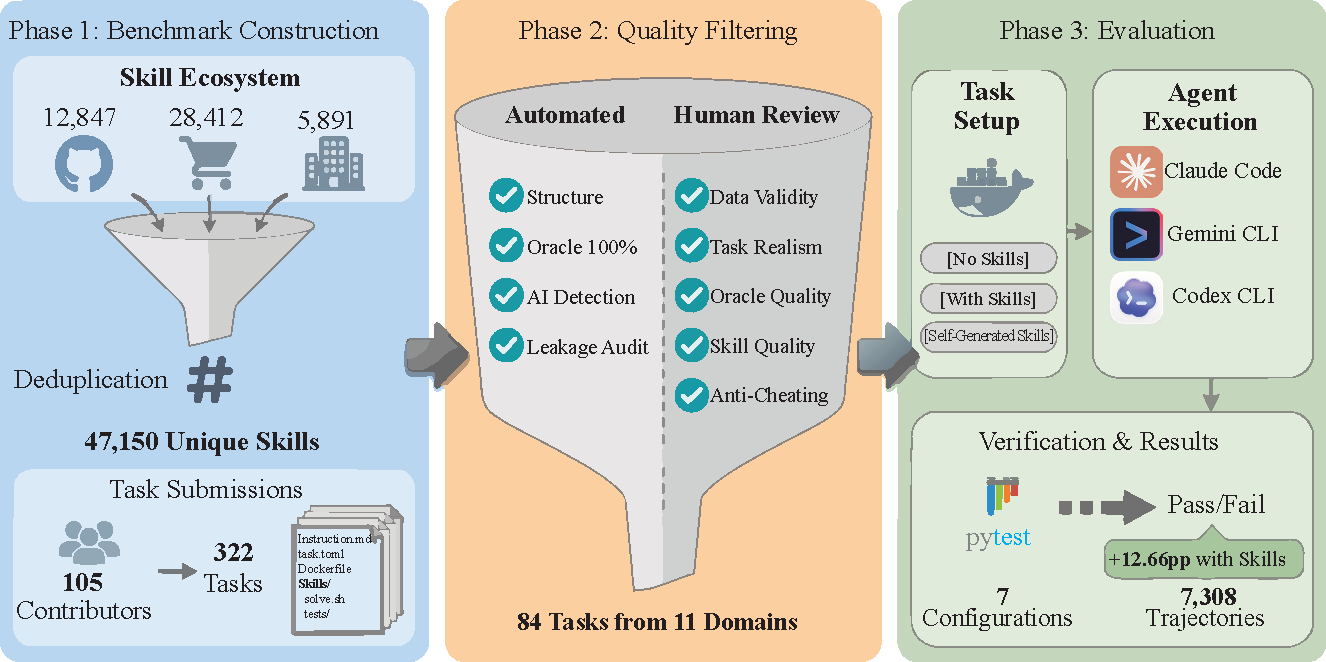
\includegraphics[width=\textwidth]{figs/pipeline.pdf}}
    \caption{\textbf{\benchmarkName{} pipeline overview.}
    \textbf{Phase~1 (Benchmark Construction):} We aggregate Skills from three sources---open-source repositories (12,847), the Claude Code ecosystem (28,412), and corporate partners (5,891)---yielding 47,150 unique Skills after deduplication. In parallel, 322 contributors submit 105 candidate tasks.
    \textbf{Phase~2 (Quality Filtering):} Each task undergoes automated checks (structural validity, AI detection, leakage audit) and human review (data validity, task realism, oracle quality, Skill quality, anti-cheating), producing 84 tasks spanning 11 domains.
    \textbf{Phase~3 (Evaluation):} Tasks are executed under three conditions (no Skills, with curated Skills, self-generated Skills) across three commercial agent harnesses (Claude Code, Gemini CLI, Codex CLI). Deterministic \texttt{pytest} verifiers produce pass/fail outcomes; 7 agent-model configurations yield 7,308 trajectories, with curated Skills providing +12.66pp average improvement.}
    \label{fig:pipeline}
  \end{center}
  \vskip -0.2in
\end{figure*}

\paragraph{Leakage Prevention.}
\label{sec:leakage}
To prevent Skills from encoding task-specific solutions, we enforce explicit authoring guidelines and conduct leakage audits.
A Claude Code Agent SDK-based validation agent runs in CI to detect potential Skill-solution leakage; failed tasks are rejected.
Skills must NOT contain: task-specific filenames, paths, or identifiers; exact command sequences that solve benchmark tasks; constants, magic numbers, or values from task specifications; references to specific test cases or expected outputs.
Skills must be applied to a class of tasks, not a single instance; provide procedural guidance (how to approach), not declarative answers (what to output); and be authored independently of benchmark specifications.


% \paragraph{Automated Validation.}
% Each submission undergoes automated validation before human review: structural validation (required files present, correct directory layout, valid syntax), oracle execution (reference solution must achieve 100\% test pass rate), instruction being human written (we apply both human review and GPTZero review, and we achieve human label on 100\% of our tasks), and instruction quality assessment against six criteria (explicit output paths, structured requirements, success criteria, constraints listed, context-first ordering).

% \paragraph{Human Review.}
% After automated checks pass, maintainers evaluate: (1) data validity: input data must reflect real-world complexity, (2) task realism: scenarios must reflect realistic professional workflows without artificial difficulty, (3) oracle quality---solutions should match how domain experts would solve the task, (4) Skill quality---Skills must be error-free and useful beyond this benchmark, and (5) anti-cheating---tasks must prevent shortcut solutions. Reviewers run benchmark experiments with and without Skills to confirm each task provides meaningful signal.

% \paragraph{Leakage Prevention.}
% \label{sec:leakage}
% To prevent Skills from encoding task-specific solutions, we enforce authoring guidelines and conduct leakage audits via CI. Skills must NOT contain: task-specific filenames or identifiers, exact command sequences that solve benchmark tasks, constants or values from task specifications, or references to expected outputs. Skills must apply to a class of tasks, provide procedural guidance (how to approach) rather than declarative answers (what to output), and be authored independently of benchmark specifications.


% \subsubsection{Leakage Prevention}
% \label{sec:leakage}

% To prevent Skills from encoding task-specific solutions, we enforce explicit authoring guidelines and conduct leakage audits.
% During the task collection process,
% we run a Claude Code Agent SDK-based \texttt{contribution-agent} in CI to detect potential Skills solution leakage. Tasks doesn't pass the CI will not be accepted. After the CI, each task will receive rigorous human reviews, with each PR taking at least 30 minutes from the reviewers.

% \textbf{Prohibited Content.}
% Skills must NOT contain: task-specific filenames, paths, or identifiers; exact command sequences that solve benchmark tasks; constants, magic numbers, or values from task specifications; references to specific test cases or expected outputs.

% \textbf{Required Generality.}
% Skills must: apply to a class of tasks, not a single instance; provide procedural guidance (how to approach), not declarative answers (what to output); be authored independently of benchmark specifications.

% \paragraph{Leakage Audit.} Reviewers
% We measure Skills-solution similarity using three metrics:
% \begin{enumerate}[nosep,leftmargin=*]
%     \item \textbf{N-gram overlap:} Jaccard similarity between Skills content and oracle solution ($J_{3\text{-gram}}$)
%     \item \textbf{Semantic similarity:} Embedding cosine similarity using text-embedding-3-large
%     \item \textbf{Command overlap:} Fraction of oracle commands appearing verbatim in Skills
% \end{enumerate}

% \begin{table}[h]
% \centering
% \small
% \caption{Skills leakage audit results. Low similarity scores indicate Skills provide procedural guidance rather than task-specific solutions.}
% \label{tab:leakage}
% \begin{tabular}{lccc}
% \toprule
% \textbf{Metric} & \textbf{Mean} & \textbf{Max} & \textbf{Excluded} \\
% \midrule
% N-gram Jaccard & 0.08 & 0.24 & 0 \\
% Semantic cosine & 0.15 & 0.29 & 0 \\
% Command overlap & 0.12 & 0.31 & 2 \\
% \bottomrule
% \end{tabular}
% \end{table}

% Skills with any similarity metric $> 0.30$ were revised or excluded.



\subsection{Benchmark Composition}

\begin{table}[t]
\centering
\small
\caption{Task difficulty stratification based on human completion time.}
\label{tab:levels}
\begin{tabular}{lccc}
\toprule
\textbf{Difficulty} & \textbf{Tasks} & \textbf{Human Time}  \\
\midrule
Core & 17 (19.8\%) & $<$60 min\\
Extended & 43 (50.0\%) & 1--4 hours\\
Extreme & 26 (30.2\%) & $>$4 hours \\
\bottomrule
\end{tabular}
\end{table}

% \begin{table}[t]
% \centering
% \small
% \caption{Task difficulty stratification based on human completion time.}
% \label{tab:levels}
% \begin{tabular}{lccc}
% \toprule
% \textbf{Difficulty} & \textbf{Tasks} & \textbf{Human Time}  \\
% \midrule
% Core & 6 (7.1\%) & $<$60 min\\
% Extended & 52 (61.2\%) & 1--4 hours\\
% Extreme & 27 (31.8\%) & $>$4 hours \\
% \bottomrule
% \end{tabular}
% \end{table}

% \benchmarkName{} comprises 85 tasks across 13 domains, with category distribution shown in \autoref{fig:category_distribuion}.
% We stratify tasks by difficulty, measured by estimated completion time by individuals who are considered median specialists for the tasks, without the assistance of AI tools. Original task contributors provided human time estimates, reviewed by an additional set of reviewers from the maintainers who are expert in the same domain. 

\benchmarkName{} comprises 84 tasks across 11 domains, with category distribution shown in \autoref{fig:category_distribuion}.
%We exclude two tasks (\texttt{fix-visual-stability} due to verifier timeout and \texttt{mhc-layer-impl} due to GPU infrastructure requirements) from all experiments, yielding 84 evaluated tasks.
We stratify tasks by difficulty, measured by estimated completion time by individuals whom we consider median specialists for the tasks, without the assistance of AI tools. Original task contributors provided human time estimates, reviewed by an additional set of reviewers from the maintainers who are experts in the same domain.

% We supplement human time with intrinsic difficulty indicators: (1) \emph{dependency depth}---number of sequential steps requiring prior step completion (Easy: 2.1, Medium: 4.8, Hard: 8.3 mean), (2) \emph{tool invocations}---expected distinct commands (Easy: 5.2, Medium: 14.7, Hard: 28.4 mean), and (3) \emph{state complexity}---number of files/configurations modified (Easy: 2.8, Medium: 7.1, Hard: 15.2 mean).
% These metrics correlate with human time ($r = 0.73$) and provide model-agnostic difficulty characterization.

% \begin{figure}[t]
%   \vskip 0.1in
%   \begin{center}
% \centerline{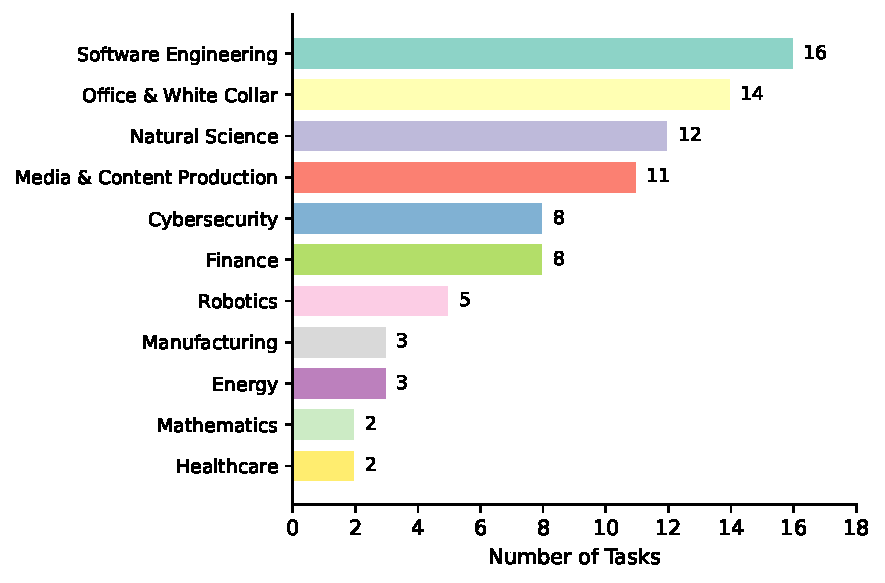
\includegraphics[width=1\columnwidth]{figs/category_distribution.pdf}}
%     \caption{\benchmarkName{} consists of tasks spanning 11 domains.}
%     \label{fig:category_distribuion}
%   \end{center}
%   \vskip -0.2in
% \end{figure}

\begin{figure}[t]
  \vskip -0.1in
  \begin{center}
\centerline{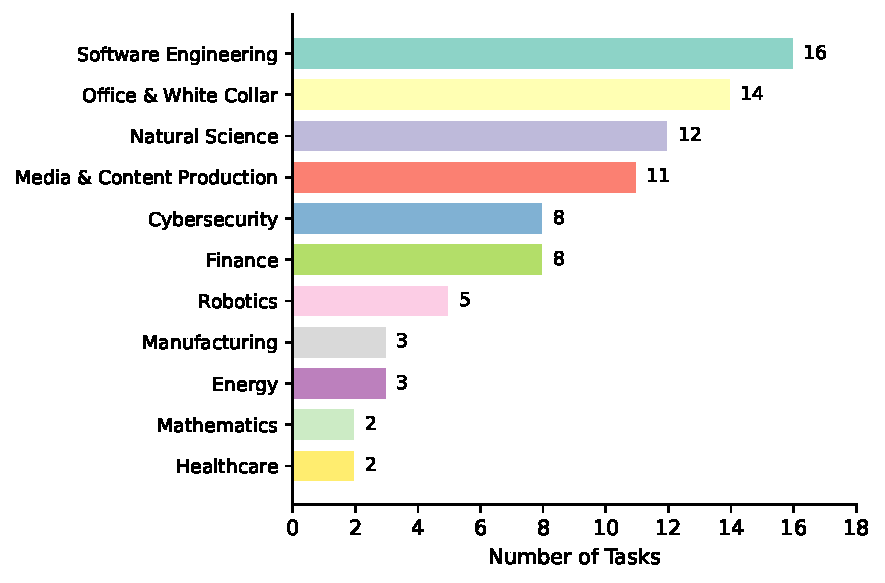
\includegraphics[width=1\columnwidth]{figs/category_distribution.pdf}}
    \caption{\benchmarkName{} consists of tasks spanning 11 domains.}
    \label{fig:category_distribuion}
  \end{center}
  \vskip -0.5in
\end{figure}

% The tasks span 13 domains: \textbf{General} (17), \textbf{Data Processing} (11), \textbf{Scientific Computing} (10), \textbf{Security} (7), \textbf{Multimedia} (7), \textbf{Financial} (7), \textbf{Control Systems} (6), \textbf{Document Processing} (5), \textbf{Software Engineering} (5), \textbf{Planning \& Optimization} (4), \textbf{Manufacturing} (3), \textbf{Web Performance} (2), and \textbf{Healthcare} (1).

% \subsection{Skills-Task Pairing}
% \label{sec:pairing}

% \paragraph{Pairing Process.}
% Each task is paired with 1--3 relevant Skills (221 total, 2.6 per task average) from public repositories.
% Pairing follows a two-stage process: (1) \emph{domain matching}---two annotators independently identify Skills whose domain tag (e.g., ``git'', ``docker'', ``testing'') matches the task category, \emph{without seeing task details}; (2) \emph{relevance filtering}---a third annotator (blind to task solutions) confirms each Skills provides procedural guidance applicable to the task \emph{class}, not the specific instance.
% Skills are selected based on domain relevance rather than task-specific fit.
% Crucially, Skills are authored independently of benchmark tasks---they existed in public repositories before benchmark construction.

% \paragraph{Skills Quality Variance.}
% Not all Skills are equally effective.
% Per-Skills efficacy (mean $\Delta$ when that Skills is present) ranged from +8.2pp to +31.4pp (median: +17.1pp).
% Three Skills (6\%) showed negative efficacy on at least one model, suggesting low-quality Skills can hurt performance.
% We identify quality predictors: Skills with explicit step-by-step procedures (+4.2pp vs.\ high-level guidance), code examples (+3.1pp), and modular structure (+2.8pp) show higher efficacy.

% \subsection{Evaluation Protocol}
% \label{sec:protocol}



% This 3-condition design enables dose-response analysis of Skills efficacy. For each condition, the agent interacts with the containerized environment until task completion, timeout, or round limit. The verifier then executes deterministic assertions to produce a binary pass/fail outcome.